\documentclass[11pt,a4paper]{article}
\usepackage[utf8]{inputenc}
\usepackage[T1]{fontenc}
\usepackage[spanish,es-noshorthands]{babel}
\usepackage{amsmath,amssymb,amsthm}
\usepackage{bm}
\usepackage{geometry}
\geometry{margin=2.5cm}
\usepackage{graphicx}
\graphicspath{{../figuras/}}
\usepackage{float}
\usepackage{xcolor}
\usepackage{hyperref}
\hypersetup{colorlinks=true,linkcolor=blue!50!black,citecolor=blue!50!black,urlcolor=blue!50!black}
\usepackage{enumitem}
\usepackage{booktabs}
\newtheorem{definition}{Definición}
\newtheorem{remark}{Observación}
\newcommand{\R}{\mathbb{R}}
\newcommand{\thetavec}{\bm{\theta}}
\newcommand{\transp}{^{\top}}
\newcommand{\promptIA}[1]{\begin{center}\fcolorbox{gray}{gray!8}{\parbox{0.9\linewidth}{\small\textbf{[FIGURA -- PROMPT IA]}\\[2pt]#1}}\end{center}}
\title{\textbf{Ecuaciones diferenciales y sistemas dinámicos}\\[2pt]\large La lente para leer Wilson--Cowan como sistema dinámico (M2)}
\author{Proyecto Wilson--Cowan --- Iniciación a la I+D ITBA}
\date{\today}
\begin{document}
\maketitle
\tableofcontents
\bigskip

\section*{Antes de empezar}
\addcontentsline{toc}{section}{Antes de empezar}
Este documento (M2) asume que ya leíste M1 (álgebra lineal: vectores, matrices, autovalores, Jacobiano). Acá no volvemos a explicar qué es una derivada ni qué es un autovalor; lo que hacemos es \emph{poner esas piezas a trabajar} sobre un sistema que evoluciona en el tiempo. El objetivo concreto: darte el vocabulario y las herramientas para mirar el modelo de Wilson--Cowan (WC, ver B3) no como un par de fórmulas sueltas, sino como un \emph{sistema dinámico} cuyo comportamiento (reposo, oscilación, ritmo theta--gamma) se lee en un dibujo. Todo el documento usa WC como ejemplo recurrente.

\section{Qué es una EDO: problema de valor inicial, campo vectorial y flujo}

\begin{definition}[Ecuación diferencial ordinaria]
Una EDO de primer orden es una regla que dice cuánto vale la \emph{tasa de cambio} de un estado en función del estado actual (y quizás del tiempo):
\begin{equation}
\dot{\mathbf{x}}(t) = \mathbf{f}(\mathbf{x}(t),\,t), \qquad \mathbf{x}\in\R^n,
\end{equation}
donde $\dot{\mathbf{x}} = \mathrm{d}\mathbf{x}/\mathrm{d}t$. La función $\mathbf{f}$ es el \emph{campo vectorial}: en cada punto del espacio te dice hacia dónde y con qué velocidad se mueve el estado.
\end{definition}

\paragraph{Intuición.} Una EDO no te da directamente la trayectoria; te da la \emph{ley de movimiento}. Es como estar parado en un río: en cada punto el agua tiene una velocidad (eso es $\mathbf{f}$). Si soltás un corcho en una posición inicial $\mathbf{x}(t_0)=\mathbf{x}_0$, la corriente lo arrastra por un único camino. Ese ``dónde arranco + la ley del río'' es el \textbf{problema de valor inicial} (PVI):
\begin{equation}
\dot{\mathbf{x}} = \mathbf{f}(\mathbf{x},t), \qquad \mathbf{x}(t_0)=\mathbf{x}_0.
\end{equation}
Bajo condiciones suaves (que $\mathbf{f}$ sea Lipschitz, cumplido de sobra por WC porque las sigmoideas son suaves), el PVI tiene \emph{solución única}. Esa unicidad es la que hace que el modelo sea determinista: mismos parámetros y misma condición inicial $\Rightarrow$ misma trayectoria.

\paragraph{Flujo.} A la aplicación que toma la condición inicial $\mathbf{x}_0$ y devuelve dónde está el estado tras un tiempo $t$ se la llama \emph{flujo}, $\phi_t(\mathbf{x}_0)$. El corcho a los 3 segundos está en $\phi_3(\mathbf{x}_0)$.

\paragraph{Por qué en este proyecto.} WC \emph{es} una EDO. Su estado es $\mathbf{x}=[I,E]$ (las tasas de disparo, \emph{firing rate}, de las poblaciones inhibitoria y excitatoria), y su campo vectorial es, en la forma canónica del proyecto (con $S_a(u)=1/(1+e^{-au})$):
\begin{align}
\dot I &= \tfrac{1}{\tau_i}\big(-I + S_i(w_{IE}E - w_{II}I + Q(t) - \theta_i) - k_i\big),\label{eq:wc_I}\\[2pt]
\dot E &= \tfrac{1}{\tau_e}\big(-E + S_e(w_{EE}E - w_{EI}I + P(t) - \theta_e) - k_e\big),\label{eq:wc_E}
\end{align}
con $k_e = 1/(1+e^{a_e\theta_e})$ y $k_i = 1/(1+e^{a_i\theta_i})$. Los offsets $k_e,k_i$ se restan para que el reposo $E=I=0$ sea equilibrio sin estímulo (se \emph{derivan}, no se aprenden libres). La salida observada es $y(t)=E(t)-I(t)$, y $P(t)\!\to\!E$, $Q(t)\!\to\!I$ son los estímulos externos. Identificar el modelo (P4) es, en el fondo, encontrar los 10 parámetros $\thetavec$ que hacen que el flujo de esta EDO reproduzca los datos.

\section{Espacio de estados y retrato de fase (foco en 2D)}

\begin{definition}[Espacio de estados]
Es el espacio $\R^n$ donde vive el estado $\mathbf{x}$. Cada punto es una ``foto'' completa del sistema en un instante; una trayectoria es una curva que recorre ese espacio a medida que pasa el tiempo.
\end{definition}

Para WC, $n=2$: el espacio de estados es el plano $(I,E)$. Esto es una suerte enorme, porque \textbf{el caso 2D se dibuja}. El dibujo de las trayectorias en ese plano se llama \emph{retrato de fase} (\emph{phase portrait}).

\paragraph{Intuición.} En el retrato de fase el tiempo desaparece del eje: no ves ``valor vs tiempo'' sino ``$I$ vs $E$''. Sobre él se dibuja el campo vectorial como un campo de flechitas (cada flecha es $\mathbf{f}$ en ese punto), y las trayectorias son las curvas tangentes a esas flechas. Una cosa que parece una serie temporal complicada (subibaja de $E$ y de $I$) puede ser, en el plano, algo tan simple como una curva cerrada que se recorre una y otra vez.

\paragraph{Por qué en este proyecto.} Todo el comportamiento cualitativo de WC ---si se queda quieto, si oscila, con qué amplitud--- se \emph{lee} en el retrato de fase del plano $[I,E]$. La Figura~\ref{fig:retrato} es exactamente ese dibujo para los parámetros del proyecto. Es la herramienta central de M2 y la razón de que este documento exista: convierte ``resolver una EDO'' en ``mirar una geometría''.

\section{Puntos de equilibrio, linealización y clasificación por autovalores}

\begin{definition}[Punto de equilibrio]
Un punto $\mathbf{x}^{*}$ es un equilibrio (o punto fijo) si el campo vectorial se anula ahí: $\mathbf{f}(\mathbf{x}^{*})=\mathbf{0}$. Si el estado arranca exactamente en $\mathbf{x}^{*}$, se queda ahí para siempre: $\dot{\mathbf{x}}=\mathbf{0}$.
\end{definition}

\paragraph{Intuición.} Los equilibrios son los ``lugares donde el río está quieto''. Pero quieto no quiere decir estable: una pelota en el fondo de un pozo y una pelota en la punta de un cerro están ambas en equilibrio, pero se comportan al revés ante un empujoncito. Para distinguir uno del otro miramos qué hace el sistema \emph{cerca} del equilibrio, y ahí entra la \textbf{linealización}.

\paragraph{Linealización: el Jacobiano de estado.} Cerca de $\mathbf{x}^{*}$ aproximamos el campo por su derivada. La derivada de una función vectorial respecto del estado es una matriz: el \emph{Jacobiano de estado}
\begin{equation}
J(\mathbf{x}^{*}) = \frac{\partial \mathbf{f}}{\partial \mathbf{x}}\bigg|_{\mathbf{x}^{*}}
= \begin{bmatrix}
\dfrac{\partial \dot I}{\partial I} & \dfrac{\partial \dot I}{\partial E}\\[8pt]
\dfrac{\partial \dot E}{\partial I} & \dfrac{\partial \dot E}{\partial E}
\end{bmatrix}_{\mathbf{x}^{*}}.
\end{equation}
Escribiendo la perturbación $\bm{\delta}=\mathbf{x}-\mathbf{x}^{*}$, cerca del equilibrio el sistema se comporta como el sistema \emph{lineal} $\dot{\bm{\delta}}\approx J\,\bm{\delta}$.

\begin{remark}
Ojo con la notación, porque en este proyecto hay \emph{dos} Jacobianos distintos y conviene no confundirlos. El de acá es $\partial\mathbf{f}/\partial\mathbf{x}$ (derivada respecto del \emph{estado} $[I,E]$): gobierna la \emph{dinámica} y la estabilidad. El que aparece en identificabilidad (Fisher, M-posterior) es la sensibilidad de la salida respecto de los \emph{parámetros}, $\partial y/\partial\thetavec$: gobierna qué tan bien se \emph{estiman} los parámetros. Distinta cosa; misma palabra.
\end{remark}

\paragraph{Clasificación por autovalores.} La dinámica lineal $\dot{\bm{\delta}}=J\bm{\delta}$ está dictada por los autovalores $\lambda_{1,2}$ de $J$ (ver M1). En 2D:
\begin{itemize}[nosep,leftmargin=1.4em]
\item \textbf{Nodo:} autovalores reales del mismo signo. Trayectorias que entran (si $<0$, estable) o salen (si $>0$) sin girar.
\item \textbf{Foco (espiral):} autovalores complejos conjugados $\lambda=\alpha\pm i\beta$. Hay giro (por la parte $\beta$) más contracción o expansión (por la parte $\alpha$). Estable si $\alpha<0$ (espiral que cae al equilibrio).
\item \textbf{Silla (\emph{saddle}):} autovalores reales de signos opuestos. Atrae por una dirección y repele por otra: inestable.
\item \textbf{Centro:} autovalores imaginarios puros $\lambda=\pm i\beta$ ($\alpha=0$). Órbitas cerradas alrededor del equilibrio; caso frontera, no robusto.
\end{itemize}

\paragraph{Por qué en este proyecto.} El mismo WC, con los mismos 10 pesos, cambia de tipo de equilibrio según el estímulo. Dato del proyecto (SPEC \S5): con $P\!\approx\!1.2,\,Q\!\approx\!0.6$ el equilibrio pierde estabilidad y aparece una oscilación; con $P\!=\!0.8,\,Q\!=\!0.6$ el sistema cae en un \emph{foco estable} (espiral que se apaga, sin ritmo). Es literalmente el mismo modelo: lo que cambia es dónde caen los autovalores de $J$. Saber leer eso es saber predecir si WC va a oscilar o no.

\section{Estabilidad y nulclinas}

\paragraph{Estabilidad.} La regla operativa sale directo de los autovalores de $J(\mathbf{x}^{*})$: el equilibrio es \textbf{asintóticamente estable} si \emph{todas} las partes reales son negativas ($\mathrm{Re}\,\lambda_i<0$), e \textbf{inestable} si al menos una es positiva. La parte imaginaria solo dice si el acercamiento (o alejamiento) es en espiral o derecho. El signo de la parte real es el interruptor de encendido/apagado del sistema; guardá esta idea, porque la bifurcación de Hopf (\S5) es exactamente el instante en que ese signo cruza el cero.

\begin{definition}[Nulclina]
La \emph{nulclina} de una variable es el conjunto de puntos del espacio de estados donde su derivada se anula. En WC hay dos:
\begin{align*}
\text{nulclina de } E:&\quad \dot E = 0 \;\Longrightarrow\; E = S_e(w_{EE}E - w_{EI}I + P - \theta_e) - k_e,\\
\text{nulclina de } I:&\quad \dot I = 0 \;\Longrightarrow\; I = S_i(w_{IE}E - w_{II}I + Q - \theta_i) - k_i.
\end{align*}
\end{definition}

\paragraph{Intuición.} Sobre la nulclina de $E$ la variable $E$ no crece ni decrece (las flechas del campo apuntan verticalmente); sobre la de $I$, $I$ está congelada (flechas horizontales). Donde las dos nulclinas \emph{se cruzan}, ambas derivadas son cero a la vez: eso es un equilibrio. Por eso las nulclinas son la forma práctica de \emph{encontrar} los equilibrios sin resolver nada numéricamente: los dibujás y buscás las intersecciones. Su forma de S (heredada de la sigmoidea) y cómo se cruzan determinan cuántos equilibrios hay y de qué tipo.

\paragraph{Por qué en este proyecto.} En la Figura~\ref{fig:retrato} las dos nulclinas están dibujadas sobre el retrato de fase de WC. La geometría de su cruce ---en particular que se corten en la ``rama del medio'', la de pendiente positiva de la nulclina de $E$--- es la firma de que el equilibrio es inestable y de que el sistema, en vez de quedarse ahí, se va a la oscilación. Nulclinas + campo vectorial + trayectoria son las tres capas de ese único dibujo.

\begin{figure}[H]
\centering
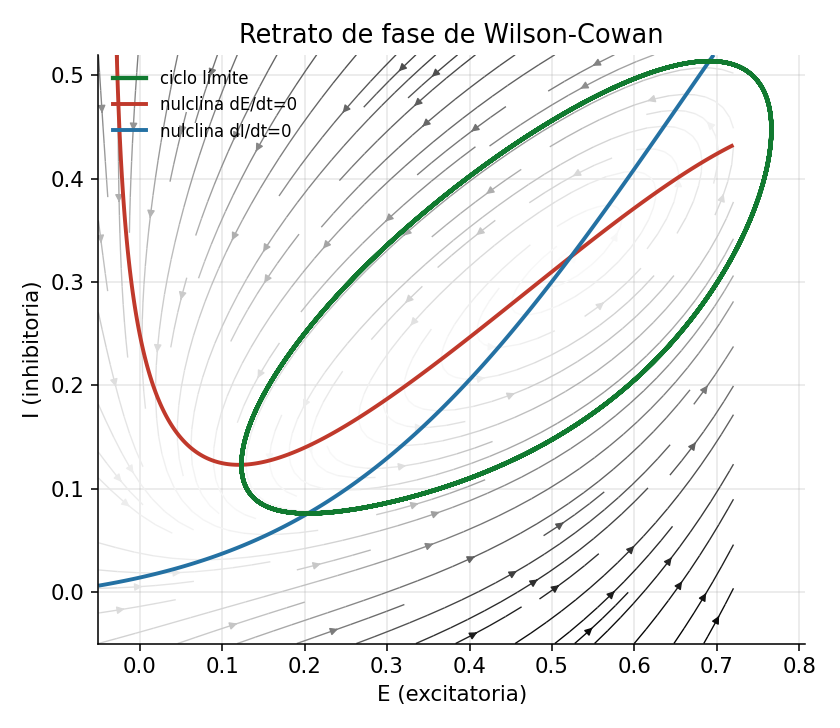
\includegraphics[width=0.75\linewidth]{fig_retrato_fase_wc.png}
\caption{Retrato de fase de Wilson--Cowan en el plano de estados $[I,E]$ para el régimen oscilatorio ($P\!\approx\!1.2,\,Q\!\approx\!0.6$): campo vectorial (flechas), las dos nulclinas ($\dot E=0$ y $\dot I=0$) y la trayectoria. El cruce de las nulclinas es un equilibrio \emph{inestable}: en vez de caer ahí, la trayectoria se enrolla hacia una curva cerrada, el \textbf{ciclo límite}. Ese lazo cerrado \emph{es} la oscilación: cada vuelta completa del estado por el lazo corresponde a un período del ritmo. Comparar con la Figura~\ref{fig:series}, que muestra la misma solución desplegada en el tiempo. (figura del proyecto)}
\label{fig:retrato}
\end{figure}

\section{Oscilaciones, ciclo límite y bifurcación de Hopf}

\begin{definition}[Ciclo límite]
Un \emph{ciclo límite} (\emph{limit cycle}) es una trayectoria cerrada \emph{aislada} del espacio de estados hacia la cual convergen las trayectorias vecinas. Cerrada = periódica (el estado vuelve al mismo punto); aislada = no hay una familia continua de órbitas alrededor (eso la distingue del centro).
\end{definition}

\paragraph{Intuición.} El ciclo límite es una oscilación \emph{autosostenida y robusta}. A diferencia del centro (donde la amplitud depende de dónde arrancaste y cualquier empujón la cambia para siempre), el ciclo límite tiene amplitud y período propios: si lo perturbás, el sistema vuelve solo al mismo lazo. Es la firma matemática de un ``reloj'' interno. En el retrato de fase se ve como un rulo cerrado al que todo cae; en el tiempo se ve como una oscilación de amplitud fija (Figura~\ref{fig:series}).

\begin{figure}[H]
\centering
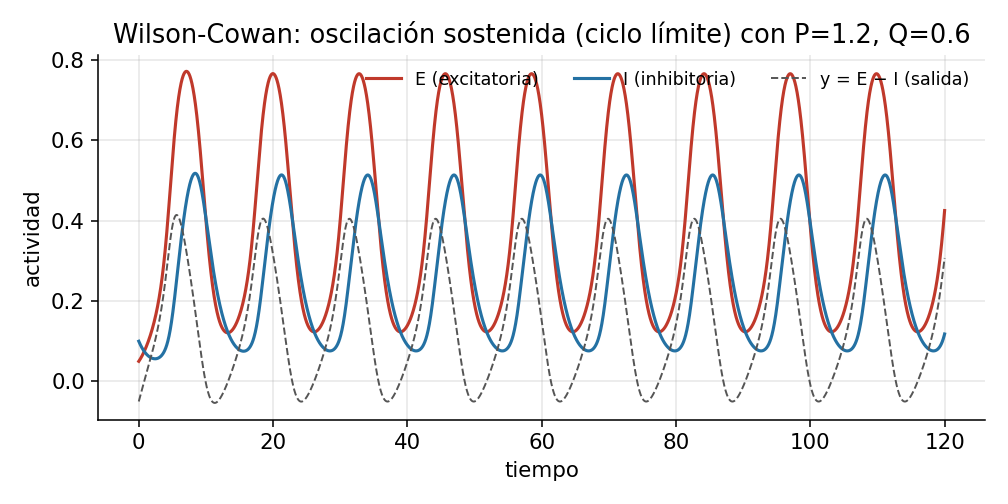
\includegraphics[width=0.75\linewidth]{fig_wc_series.png}
\caption{La misma solución de la Figura~\ref{fig:retrato}, ahora vista en el tiempo: $I(t)$, $E(t)$ y la salida observada $y=E-I$ ($P\!=\!1.2,\,Q\!=\!0.6$). La oscilación sostenida de amplitud constante es la traducción temporal del lazo cerrado del retrato de fase: \textbf{una vuelta completa por el ciclo límite = un período de estas curvas}. Un foco estable, en cambio, daría oscilaciones que se apagan hasta la línea plana. (figura del proyecto)}
\label{fig:series}
\end{figure}

\paragraph{Bifurcación de Hopf: cómo ``nace'' un ritmo.} Una \emph{bifurcación} es un cambio cualitativo del retrato de fase al variar un parámetro de control (para WC, típicamente el estímulo $P$ o $Q$). La \textbf{bifurcación de Hopf} es la que crea oscilaciones: al mover el parámetro, el par de autovalores complejos conjugados del equilibrio $\lambda=\alpha(\mu)\pm i\beta(\mu)$ cruza el eje imaginario, es decir, $\alpha$ pasa de negativo a positivo. Justo en el cruce ($\alpha=0$) el foco estable pierde la estabilidad y \emph{nace} un ciclo límite de amplitud pequeña, que crece a medida que seguís empujando el parámetro. En el instante crítico el sistema oscila con frecuencia $\beta/2\pi$: la parte imaginaria del autovalor te da la frecuencia del ritmo naciente.

\paragraph{Por qué en este proyecto: conexión explícita con B3.} Esto es \emph{el mecanismo} por el que Wilson--Cowan oscila, y es puramente el \textbf{acople excitatorio--inhibitorio (E/I)}. La idea, en cámara lenta: $E$ se autoexcita ($w_{EE}$) y activa a $I$ ($w_{IE}$); $I$, con retraso (su constante de tiempo $\tau_i=2.0$ es el doble que $\tau_e=1.0$), frena a $E$ ($w_{EI}$); al caer $E$, cae el drive sobre $I$, así que $I$ afloja y $E$ puede volver a subir. Ese lazo con retardo ---excitar, ser frenado, soltar el freno, volver a excitar--- es un oscilador. Cuando el estímulo lleva al equilibrio a través de una Hopf ($P\!\approx\!1.2,\,Q\!\approx\!0.6$), el lazo E/I ya no se estabiliza y se convierte en el ciclo límite de las Figuras~\ref{fig:retrato} y~\ref{fig:series}. Bajar el drive ($P\!=\!0.8$) devuelve al sistema al otro lado de la Hopf: foco estable, sin ritmo. En el régimen objetivo del proyecto, este mecanismo E/I es lo que produce las oscilaciones \textbf{theta--gamma} (ver B3): un ritmo rápido gamma nacido del lazo E/I, modulado por una envolvente theta más lenta. La bifurcación de Hopf es, entonces, la explicación de una línea de una frase del proyecto: ``WC oscila por el acople E/I''.

\section{Rigidez (\emph{stiffness}): por qué fija el paso de integración}

\begin{definition}[Rigidez / stiffness]
Un sistema es \emph{rígido} (\emph{stiff}) cuando su Jacobiano de estado $\partial\mathbf{f}/\partial\mathbf{x}$ tiene autovalores con partes reales de magnitudes muy dispares: unos procesos evolucionan mucho más rápido que otros. Se cuantifica con la \emph{razón de rigidez}
\begin{equation}
\kappa_{\text{stiff}} \;=\; \frac{\max_i |\mathrm{Re}\,\lambda_i|}{\min_i |\mathrm{Re}\,\lambda_i|}.
\end{equation}
\end{definition}

\paragraph{Intuición.} Imaginá una escena con un colibrí (aletea rquísimo) y una tortuga (camina lentísimo) que querés filmar juntos. La cámara tiene que muestrear tan rápido como el colibrí para no perderlo, aunque a vos solo te interese la tortuga. En una EDO pasa igual: aunque la dinámica \emph{lenta} sea la que te importa, un método explícito de integración (Euler, RK4; ver M3) tiene que usar un paso $\Delta t$ chico ligado a la componente \emph{más rápida} (el $|\mathrm{Re}\,\lambda|$ mayor), o la solución numérica explota. Por eso el autovalor de mayor magnitud de $\partial\mathbf{f}/\partial\mathbf{x}$ \emph{fija el paso máximo estable}: para métodos explícitos, aproximadamente $\Delta t \lesssim c/|\lambda_{\max}|$. Cuanto más rígido el sistema, más chico el paso obligado y más caro integrar. (El detalle de estabilidad de cada método es tema de M3; acá solo mostramos de dónde sale la restricción.)

\paragraph{Por qué en este proyecto.} Acá hay una \textbf{buena noticia concreta}: WC es un sistema \emph{poco rígido}. Sus autovalores de $\partial\mathbf{f}/\partial\mathbf{x}$ son moderados y de magnitud parecida (dato del proyecto: $|\lambda_{\max}|\approx 0.70$), en parte porque las dos constantes de tiempo, $\tau_e=1.0$ y $\tau_i=2.0$, difieren apenas por un factor $2$. Consecuencias prácticas, todas favorables para la identificación (P4):
\begin{itemize}[nosep,leftmargin=1.4em]
\item \textbf{Se admiten pasos grandes.} Con $|\lambda_{\max}|\approx0.70$ el paso estable es holgado, así que se puede integrar con $\Delta t$ amplio sin que reviente. Esto abarata el costo de simular durante el entrenamiento del Neural ODE (ver los barridos de costo vs $\Delta t$ del proyecto).
\item \textbf{No hace falta un integrador rígido.} No es obligatorio recurrir a métodos implícitos caros: RK4 explícito alcanza. Un sistema stiff (autovalores muy dispares) obligaría a lo contrario.
\item \textbf{Es un adelanto de M3}, donde se compara Euler vs RK4 y se elige el paso de integración: acá justificamos \emph{por qué} WC permite ser generoso con $\Delta t$; allá se cuantifica el trade-off exacto entre paso, costo y error.
\end{itemize}

\begin{remark}
No confundir las dos ``mediciones de mal condicionamiento'' del proyecto. La rigidez usa la razón de autovalores de $\partial\mathbf{f}/\partial\mathbf{x}$ y afecta la \emph{integración}. El mal condicionamiento de la identificabilidad usa la razón de valores singulares de la matriz de Fisher (o de $\partial y/\partial\thetavec$) y afecta la \emph{estimación de parámetros} (es de ahí que sale el cuello de botella de $w_{II}$). Que WC sea numéricamente amable para integrar no lo hace amable para identificar: son dos ejes distintos.
\end{remark}

\section*{Síntesis}
\addcontentsline{toc}{section}{Síntesis}
Un sistema dinámico se resume en su campo vectorial $\mathbf{f}$; su comportamiento cualitativo se lee en el retrato de fase (equilibrios en el cruce de nulclinas, tipo dado por los autovalores del Jacobiano de estado). WC vive en 2D, así que ese dibujo es directo: según el estímulo, el mismo modelo pasa de foco estable a ciclo límite vía una bifurcación de Hopf, y ese ciclo ---el lazo cerrado del retrato de fase--- es la oscilación E/I que produce el régimen theta--gamma (B3). Como su Jacobiano de estado es poco rígido ($|\lambda_{\max}|\approx0.70$), integrarlo es barato y admite pasos grandes, lo que prepara la elección de método y paso en M3.

\begin{thebibliography}{9}
\bibitem{strogatz} Strogatz, S. H., \emph{Nonlinear Dynamics and Chaos}, Addison--Wesley, 1994.
\bibitem{izhikevich} Izhikevich, E. M., \emph{Dynamical Systems in Neuroscience}, MIT Press, 2007.
\bibitem{ermentrout} Ermentrout, G. B. \& Terman, D. H., \emph{Mathematical Foundations of Neuroscience}, Springer, 2010.
\end{thebibliography}

\end{document}
